\documentclass[10pt]{report}
\usepackage[utf8]{inputenc}
\usepackage{titlesec}
\titleformat{\section}
  {\normalfont\Large\bfseries}
  {\thesection}{1em}{}
  [\vspace{0.5ex}\titlerule]
\usepackage{graphicx}
\usepackage{float}
\usepackage{fullpage}
\usepackage{hyperref}
\usepackage{enumitem}
\usepackage{pdfpages}
\usepackage{amsmath}
\usepackage{amssymb}
\usepackage{orcidlink}
\usepackage{color}
\usepackage{parskip}
\usepackage{xurl}
\usepackage{etoolbox}
\apptocmd{\sloppy}{\hbadness 10000\relax}{}{} % Allow more flexible line breaks
\setlist[itemize]{noitemsep, topsep=2pt}

\begin{document}

\begin{center}
    \href{https://github.com/Mohammad-Neutrino/CV}{\bf \huge Curriculum Vitae}\\[0.05cm]
    \href{https://physics.ku.edu/people/seikh-mohammad-ful-hossain}{\bf \large Mohammad Ful Hossain Seikh} ~~\textcolor{blue}{fulhossain@ku.edu}
    \rule{\textwidth}{0.4pt}
    Current: 1607 W 9th Street Apt 6B, Lawrence, KS, USA, 66044 $\vert$ +1 (785)727-6913 \\
    Permanent: Jinarapara, Saktipur, Murshidabad, WB, India, 742163 $\vert$ +91 7060617358
\end{center}

% ------------------------------
\section*{Professional Objective}
To contribute to real-world sensor algorithm development by applying my experience in Python, digital signal processing, machine learning, statistical modeling, and RF/radar waveform analysis. I am especially interested in developing, testing, and validating algorithms that turn complex measurement data into accurate and useful product-level outputs.

% ------------------------------
\section*{Education}

\noindent
\textbf{Ph.D. in Physics} \textit{2020--2026} \\
University of Kansas, USA \hfill \textbf{3.964/4.0}

\vspace{0em}
\noindent
\textbf{M.S. in Electrical Engineering}    \textit{2024--2025} \\
University of Kansas, USA \hfill \textbf{3.778/4.0}

\vspace{0em}
\noindent
\textbf{M.Sc. in Physics}  \textit{2018--2020} \\
Aligarh Muslim University, India \hfill \textbf{9.170/10} (Gold Medalist)

\vspace{0em}
\noindent
\textbf{B.Sc. Honors in Physics}  \textit{2015--2018} \\
Aligarh Muslim University, India \hfill \textbf{9.186/10} (Gold Medalist)

\vspace{0em}
\noindent
\textbf{Higher Secondary (12th)}  \textit{2014} \\
Central Board of Secondary Education, India \hfill \textbf{9.120/10} (First Position)

\vspace{0em}
\noindent
\textbf{Secondary (10th)} \textit{2012} \\
Central Board of Secondary Education, India \hfill \textbf{10/10} (Certificate of Merit)

% ------------------------------
\section*{Research Experience}

\subsection*{Selected Dissertations, Theses, and Projects}
\begin{itemize}
    \item \textbf{Physics PhD Dissertation}  \textit{2020--2026} \\
    Title: ``Toward a Five-Station Diffuse Ultra-High Energy Neutrino Search with the Askaryan Radio Array: ARA01 Analysis Framework". Defended on May 8, 2026. Advised by Prof.\ D. Besson. 
    
    \item \textbf{Electrical Engineering Master's Project}  \textit{2024--2025} \\
     Developed \textbf{AAFIYA}: \textbf{A}ntenna \textbf{A}nalysis in \textbf{F}requency-domain for \textbf{I}mpedance and \textbf{Y}ield \textbf{A}ssessment, a modular Python toolkit for rigorous, reproducible analysis and visualization of antenna S-parameters, impedance, and gain/beam patterns from both measurement and simulation data, with Prof.\ Jim Stiles at EECS Department, KU, (\href{https://drive.google.com/file/d/16pZq9mp9qqmyMbJ__h_DtHzoyZJUpfUi/view?usp=share_link}{Report}), (\href{https://drive.google.com/file/d/1gTU03rgjUmX7zF2z2f57pjpDCmZjiHhI/view?usp=share_link}{Slides}).

     \item \textbf{Physics Master's Thesis}  \textit{2019--2020} \\
     Investigated light sterile neutrino oscillations with Prof.\ M.S. Athar at Aligarh Muslim University (AMU), producing review report ``Light Sterile Neutrinos: Status and Prospects'' (\href{https://www.researchgate.net/publication/354254795_LIGHT_STERILE_NEUTRINOS_OSCILLATION_STATUS_AND_PROSPECTS}{DOI:10.13140/RG.2.\\2.13777.66405}).

     \item \textbf{Physics Undergraduate Project}  \textit{2017--2018} \\
     ``Quarks \& Leptons'': Detailed study of Standard Model interactions with Prof.\ M.S. Athar at AMU \href{https://drive.google.com/file/d/11LsyY1QmncnjOGf1ZWpj7eTM-xcTbCNj/view?usp=sharing}{[Handwritten Report]}.

\end{itemize} 

\subsection*{Research Roles and Appointments}
\begin{itemize}

    \item \textbf{Primary Analyzer, Askaryan Radio Array (ARA) Station 1}  \textit{2021--Present} \\
    Conducting data analysis of ARA Station 1 for ultra-high energy (UHE) neutrino detection with Prof.\ D. Besson at University of Kansas (KU).

    \item \textbf{Analysis Lead, Radio Background Characterization with ARA}  \textit{Dec 2025--Present} \\
    Leading the analysis of astrophysical, environmental, and anthropogenic radio backgrounds in ARA data with Prof.\  D. Besson at KU.

    \item \textbf{IceCube Neutrino Observatory Monitoring}  \textit{2021--Present} \\
    Served as KU representative for monitoring shifts, presenting weekly reports to the collaboration.

    \item \textbf{Machine Learning Project}  \textit{2025} \\
    Developed a CNN model for ``Automatic Surface Detection in Echograms using Deep Learning'' as a part of Machine Learning class at EECS Department, KU, (\href{https://github.com/Mohammad-Neutrino/Machine_Learning_Project}{Project Repository}), (\href{https://github.com/Mohammad-Neutrino/Machine_Learning_Project/blob/trunk/Project/report/final_report.pdf}{Report}).

    \item \textbf{Visiting Summer Student Program}  \textit{May--Jul 2019} \\
    Studied the role of $\theta_{13}$ mixing angle in three-flavor neutrino oscillations with Prof.\ S.K. Agarwalla at Institute of Physics, India, producing technical report ``Importance of 1-3 Mixing Angle in Three-Flavor Neutrino Oscillations Paradigm'' (\href{https://www.researchgate.net/publication/340095776_Importance_of_1-3_Mixing_Angle_in_Three-Flavor_Neutrino_Oscillations_Paradigm_SSVP_Summer_Project_Report}{DOI: 10.13140/RG.2.2.34421.12009}).

    \item \textbf{Winter Internship Program}  \textit{Dec 2019--Jan 2020} \\
    Researched ``Weak Interaction Physics'' at IIT-BHU with Dr. G. Abbas.
    
\end{itemize} 

% ------------------------------
\section*{Field Experience}

\noindent
\textbf{NSF's Summit Station, Greenland Field Campaign} \textit{Apr--May 2025} \\
Participated in the Radio Neutrino Observatory -- Greenland (RNO-G) calibration campaign, performing in-situ radio-frequency measurements and equipment deployment at Summit Station, Greenland.


% ------------------------------
\section*{Publications}
\subsection*{First-Author Works}
\begin{itemize}
    \item \textbf{Seikh, M.F.H., Jarvis, R., \& Stiles, J.} {\it (2026)}. ``AAFIYA: Antenna Analysis in Frequency-domain for Impedance and Yield Assessment". \href{https://doi.org/10.48550/arXiv.2601.13583}{arXiv:2601.13583 (Accepted in 2026 IEEE AP-S/URSI Symposium)}

    \vspace{0.1em}
    \noindent
    \item \textbf{Seikh, M.F.H. \& Besson, D.} {\it (2026)}. ``Polar Ice as a Laboratory for Physics". \href{https://drive.google.com/file/d/1eny09TjrDmNsoqKf86RbFbMdMi_LdEsB/view?usp=share_link}{\textit{Page 27-37, Physics Bulletin 2026, Physics Department, AMU}}

    \vspace{0.1em}
    \noindent
    \item \textbf{Seikh, M.F.H.} {\it (2025)}. ``A geometrical approach to neutrino oscillation parameters". {\it AIP Advances 1 October 2025; 15 (10): 105204}. \href{https://doi.org/10.1063/5.0292233}{DOI:10.1063/5.0292233}.

    \vspace{0.1em}
    \noindent
    \item {\bf Seikh, M.F.H., Grachev, V., Kravchenko, I., Athar, M.S., \&  Besson, D.} {\it {2025}}. ``First Radio Neutrino \& Cosmic Rays Astronomy Workshop in India". \textit{European Physics Journal-Special Topics (EPJ-ST)}. \href{https://arxiv.org/abs/2509.20704}{arXiv:2509.20704} \href{https://doi.org/10.1140/epjs/s11734-025-01955-8}{DOI:10.1140/epjs/s11734-025-01955-8}.

    \vspace{0.1em}
    \noindent
    \item {\bf Seikh, M.F.H., Giri, P. \& Besson, D. for the ARA Collaboration} {\it {2025}}. ``Techniques for Continuous Wave Identification and Filtering in the Askaryan Radio Array". \href{https://pos.sissa.it/501/1171/pdf}{PoS(ICRC2025)1171}. \href{https://arxiv.org/abs/2509.20735}{arXiv:2509.20735}.

    \vspace{0.1em}
    \noindent
    \item {\bf Seikh, M.F.H. \& Besson, D. for the RNO-G Collaboration} {\it {2025}}. ``Observation of Radio Solar Flares in RNO-G". \href{https://pos.sissa.it/501/1365/pdf}{PoS(ICRC2025)1365}. 

    \vspace{0.1em}
    \noindent
    \item \textbf{Seikh, M.F.H.} {\it (2024)}. ``Physics of radio antennas". \textit{European Physics Journal-Special Topics (EPJ-ST)}. \href{https://arxiv.org/abs/2411.07507}{arXiv:2411.07507} \href{https://doi.org/10.1140/epjs/s11734-025-01500-7}{DOI: 10.1140/epjs/s11734-025-01500-7}
    
    \vspace{0.1em}
    \noindent
    \item \textbf{Seikh, M.F.H. for the ARA Collaboration} {\it (2024)}. ``Askaryan Radio Array: searching for the highest energy neutrinos". \textit{European Physics Journal-Special Topics (EPJ-ST)}. \href{https://arxiv.org/abs/2411.01761}{arXiv:2411.01761} \href{https://doi.org/10.1140/epjs/s11734-025-01708-7}{DOI: 10.1140/epjs/s11734-025-01708-7}

    \vspace{0.1em}
    \noindent
    \item \textbf{Seikh, M.F.H. \& Besson, D.} {\it (2024)}. ``IceCube Neutrino Observatory: A Cold Discovery Hub". \href{https://drive.google.com/file/d/1q1vm4tf2Z8iK_Iw3n3kVayBnP7K6tHQI/view?usp=sharing}{\textit{Page 14-23, Physics Bulletin 2024, Physics Department, AMU}}

    \vspace{0.1em}
    \noindent
    \item \textbf{Seikh, M.F.H. for the ARA Collaboration} {\it (2023)}. ``Calibration and Physics with ARA Station 1". \textit{PoS(ICRC2023)1163}. \href{https://arxiv.org/abs/2308.07292}{arXiv:2308.07292}
    
    \vspace{0.1em}
    \noindent    
    \item \textbf{Seikh, M.F.H.} {\it (2020)}. ``Neutrinos and the 40 Future Routes". \textit{Physics Bulletin}, Physics Department, AMU. \href{https://www.researchgate.net/publication/340272190_Neutrinos_and_the_40_Future_Routes}{DOI: 10.13140/RG.2.2.27981.10729}
\end{itemize}

% ------------------------------
\subsection*{Collaborative Works}
Full publication (includes contributions to ARA, RNO-G, ARIANNA, IceCube, IceCube Gen2, PUEO, TAROGE-M and RET collaborations) record available on:
\begin{center}
    \href{https://inspirehep.net/authors/2014116}{Inspire HEP} ;~~\href{https://scholar.google.com/citations?user=dSwfpWQAAAAJ}{Google Scholar} ;~~\href{https://www.researchgate.net/profile/Mohammad-Ful-Hossain-Seikh}{ResearchGate} ;~ORCiD \orcidlink{0000-0002-4464-7354} ;~~\href{https://www.scopus.com/authid/detail.uri?authorId=57426893600}{Scopus}
\end{center}

% ------------------------------
\section*{Professional Service}
\subsection*{Editorial}
\begin{itemize}
    \item \hyperlink{appendixpage}{\bfseries Book Editor} for Springer's EPJ-ST journal: \href{https://link.springer.com/collections/ediiddhcdc}{``Radio Detection of Ultra-high Energy Neutrino \& Cosmic Ray"} (15 articles) with M.S. Athar, D. Besson, V. Grachev, and I. Karvchenko  \textit{(2024--2025)}

    \vspace{0.1em}
    \noindent  
    \item {\bf Founder and Editor-in-Chief} of \textit{The Magnetic Monopole} e-magazine for KU's Society of Physics Students    \href{https://drive.google.com/file/d/12yfhWqUupWIPWM5WcWdIviUYbVA2GnWY/view?usp=sharing}{[View Issue]}  \textit{(June 2022)}
\end{itemize}

% ------------------------------
\subsection*{Research Article Review}
\begin{itemize}

    \item {\bf Peer Reviewer:} for World Scientific's IJMP-A journal (1 article, 2 reviews) (2025)

    \vspace{0.0em}
    \noindent  
    \item {\bf Peer Reviewer:} for Springer's EPJ-ST journal (5 articles, 11 reviews) \textit{(2024--2025)}

    \vspace{0.0em}
    \noindent  
    \item {\bf Internal ARA Collaboration Reviewer:} Pawan Giri for ARA Collaboration, ``A Comprehensive Diffuse Neutrino Search Using the Full Askaryan Radio Array", 32nd International Symposium on Lepton Photon Interactions at High Energies \textit{(November 2025)}

\end{itemize}

% ------------------------------
\subsection*{Conference Session Chair}
\begin{itemize}

    \item {\bf General Cosmology:} for APS Global Physics Summit (March 19, 2026)

    \vspace{0.0em}
    \noindent  
    \item {\bf Topical Groups Session II:} for APS Global Physics Summit (March 17, 2026)

\end{itemize}

% ------------------------------
\subsection*{Other Reviews}
\begin{itemize}

    \item {\bf REU Application Reviewer:} for KU Physics and Astronomy (10 Applications) (2025)

    \vspace{0.0em}
    \noindent  
    \item {\bf SSGSA Application Reviewer:} for SSGSA (Multiple Applications) \textit{(2021--2026)}

\end{itemize}


% ------------------------------
\subsection*{Professional Leadership/Membership}
\begin{itemize}
    \item \textbf{American Physical Society (APS)}: Graduate Student Member  
    \textit{(2020--Present)}
    \item \textbf{National Society of Black Physicists}: Student Member \textit{(2021--Present)}
    \item \textbf{Physics \& Astronomy Graduate Student Organization (GSO), KU}:
    \begin{itemize}[label={\color{black}$\checkmark$}]
        \item Graduate Students Representative - Member at Large  \textit{(2025--Present)}
        \item Graduate Students Representative - Liaison  \textit{(2024--2025)}
        \item GSO Executive Officer  \textit{(2023--2024)}
    \end{itemize}%\vspace{5mm}
    \item \textbf{Sir Syed Global Scholar Award (SSGSA)}:
    \begin{itemize}[label={\color{black}$\checkmark$}]
        \item Peer Mentor \textit{(2023--Present)}
        \item Team Lead, Promotions \& Outreach \textit{(2023--2025)}
        \item Member, Mentorship \& Applications Team \textit{(2021--2023)}
        \item AMU Campus Team Member \textit{(2019--2020)}
    \end{itemize}
    \item \textbf{Society of Physics Students, KU Chapter}: Graduate President \textit{(2021--2022)}
    \item \textbf{Sigma Pi Sigma (National Physics Honor Society)}: Lifetime Member
    \item \textbf{AMU Society of Physics}: Member \textit{(2018--Present)}
\end{itemize}

% ------------------------------
\section*{Technical Proficiencies}
\begin{itemize}
    \item \textbf{Programming Languages}: C/C++, Python, FORTRAN
    \item \textbf{Physics Software}: CERN ROOT, AraRoot, Wolfram Mathematica
    \item \textbf{Simulation Packages}: AraSim, NuRadioMC, HFSS
    \item \textbf{Operating Systems}: Linux (Ubuntu), Windows, macOS
    \item \textbf{Document Preparation}: \LaTeX, Microsoft Office Suite
\end{itemize}

% ------------------------------
\section*{Honors \& Awards}
\subsection*{Academic Honors}
\begin{itemize}
    \item \textbf{University Gold Medals}:
    \begin{itemize}[label={\color{black}$\checkmark$}]
        \item M.Sc. Physics (Top among 50 students), AMU \textit{(2020)}
        \item B.Sc. Honors Physics (Top among 120 students), AMU \textit{(2018)}
        \item Highest percentage in B.Sc. (Hons) Faculty of Science, AMU \textit{(2018)}
    \end{itemize}
    \item \textbf{Abdul Aziz Medal} for B.Sc. Physics, AMU \textit{(2018)}
    \item \textbf{Undergraduate Topper Scholarship}, UGC India \textit{(2020)}
    \item \textbf{University Merit Financial Award}, AMU \textit{(2019--2020)}
    \item \textbf{First Position} in Higher Secondary (12th) among 40 students \textit{(2014)}
    \item \textbf{Certificate of Merit} for perfect 10/10 CGPA in Secondary (10th) \textit{(2012)}
\end{itemize}

% ------------------------------
\subsection*{Fellowships \& Grants}
\begin{itemize}
    \item \textbf{Ralston Dissertation Fellowship}, KU Physics \textit{(2025--2026)}
    \item \textbf{McKeithan Summer Fellowship}, KU Physics \textit{(2025)}
    \item \textbf{Graduate Student Award for Distinguished Service}, KU \textit{(2024--2025)}
    \item \textbf{Wallace S. Strobel Scholarship}, KU EECS \textit{(2024--2025)}
    \item \textbf{Ralston Summer Fellowship}, KU Physics \textit{(2024)}
    \item \textbf{Doctoral Student Research Fund}, KU \textit{(2024)}
    \item {\bf Distinguished Students Award}, APS FIP \textit{(2021--2022)}
    \item \textbf{Carl \& Catherine Chaffee Scholarship}, KU Physics \textit{(2020--2021)}
\end{itemize}

% ------------------------------
\subsection*{Conference Travel Awards}
\begin{itemize}
    \item \textbf{Graduate Student Travel Fund}, KU Physics \textit{(2023, 2025)}
    \item \textbf{DAP Travel Grant}, APS \textit{(2024)}
    \item \textbf{DPF Travel Award}, APS \textit{(2022, 2024)}
    \item \textbf{CLAS Graduate Scholarly Development Fund}, KU \textit{(2022)}
\end{itemize}

% ------------------------------
\subsection*{Other Distinctions}
\begin{itemize}
    \item \textbf{Washington DC Scholarship}, AMU Alumni Association \textit{(2015--2019)}
    \item \textbf{Sir Syed Global Scholar Award} for prospective graduate students \textit{(2018)}
\end{itemize}

% ------------------------------
\section*{Invited Lectures, Seminars, \& Colloquia}
\begin{itemize}
    \item \textbf{Radio Engineering for Particle Astrophysics Experiments}\\
    HEP Seminar, University of Nebraska-Lincoln \textit{(March 26, 2025)}
    
    \item \textbf{Radio Engineering for Particle Astrophysics Experiments} \\
    Astroparticle Seminar, Ohio State University \textit{(January 22, 2025)}
    
    \item \textbf{Radio Engineering \& Antenna Physics} \\
    Lecture Series, IEI Summer School 2024, University of Alaska, Anchorage \textit{(July 2--5, 2024)}
    
    \item \textbf{UHE Neutrino \& Cosmic Ray Detectors} \\
    ICEHAP Seminar, Chiba University, Japan \textit{(August 9, 2023)}
    
    \item \textbf{Antenna Physics \& Measurements} \\
    Lecture Series, IEI Summer School 2023, South Dakota School of Mines \textit{(July 2--5, 2023)}
    
    \item \textbf{UHE Neutrino \& Cosmic Ray Detectors} \\
    Physics Colloquium, AMU, India \textit{(January 12, 2023)}
    
    \item \textbf{Antennas in UHE Neutrino Detectors} \\
    Particle Physics Seminar, University of Delaware \textit{(October 4, 2022)}
\end{itemize}

% ------------------------------
\section*{Outreach \& Leadership}
\begin{itemize}
    \item Co-organized and hosted India's inaugural workshop on \textbf{Radio Detection of UHE Neutrino and Cosmic Rays} at AMU \textit{(April 2024)}
    \item Conducted outreach seminar on \textbf{Physics Research Opportunities} at AMU \textit{(2021)}
    \item Participated in India's first \textbf{Science Leadership Workshop} \textit{(2020)}
    \item Volunteer for \textbf{One Person One Tree} plantation drive \textit{(2017)}
    \item Participant in \textbf{Blood Donation Camp} \textit{(2017)}
\end{itemize}

% ------------------------------
\section*{Conference Presentations}
\subsection*{Oral Presentations}
\begin{itemize}

    \item \textbf{Pioneering an Array-Wide Search for Ultra-high Energy Neutrinos with ARA} \\
    APS Global Physics Summit \textit{(March 18, 2026)}

    \item \textbf{RNO-G in-ice Antennas} \\
    RNO-G Collaboration Meeting, Uppsala University \textit{(September 9--14, 2024)}
    
    \item \textbf{Radio Frequency Instrumentation} \\
    Radio Neutrino Workshop, AMU, India \textit{(April 18--20, 2024)}
    
    \item \textbf{Towards Five Station ARA Analysis} \\
    APS April Meeting, Sacramento \textit{(April 3--6, 2024)}
    
    \item \textbf{ARA Antenna Models} \\
    ARA Collaboration Meeting, Ohio State University \textit{(March 5--8, 2024)}
    
    \item \textbf{Current Status \& Future of ARA} \\
    APS Prairie Section Meeting, University of Missouri \textit{(November 30--December 2, 2023)}
    
    \item \textbf{Introduction to Antenna Physics} \\
    RET Collaboration Meeting, Vrije University Brussels \textit{(November 8--11, 2023)}
    
    \item \textbf{Gain Calibration of RNO-G Antennas} \\
    RNO-G Fall Meeting, Penn State University \textit{(September 11--15, 2023)}

    \item \textbf{Galactic Noise in Radio Neutrino Experiments} \\
    Astro Seminar, KU \textit{(October 28, 2022)}
    
    \item \textbf{Towards ARA Station 1 Calibration} \\
    APS April Meeting, New York City \textit{(April 9--12, 2022)}
    
    \item \textbf{RNO-G Ice Calibration Planning} \\
    RNO-G Collaboration Meeting, University of Chicago \textit{(April 8, 2022)}
\end{itemize}

% ------------------------------
\subsection*{Poster Presentations}
\begin{itemize}

    \item \textbf{A Geometrical Approach to Neutrino Oscillation Parameters} \\
    APS Global Physics Summit \textit{(March 17, 2026)}
    
    \item \textbf{CW Identification \& Filtering Techniques in ARA} \\
    39th ICRC, Geneva, Switzerland \textit{(July 19, 2025)}
    
    \item \textbf{Observation of radio solar flares in RNO-G} \\
    39th ICRC, Geneva, Switzerland \textit{(July 15, 2025)}
    
    \item \textbf{Gain Measurements of LPDA Antennas} \\
    APS April Meeting, Sacramento \textit{(April 3--6, 2024)}
    
    \item \textbf{Overview of ARA Detector: Five Station Analysis} \\
    ICTS Neutrino School, India \textit{(April 22--May 3, 2024)}
    
    \item \textbf{Calibration of ARA Station 1} \\
    38th ICRC, Nagoya University, Japan \textit{(July 29, 2023)}
    
\end{itemize}

% ------------------------------
\section*{Professional Development}
\begin{itemize}
    \item \textbf{The AI Masterclass 3.0}, (Dhruv Rathee Academy, \textit{Coursework ends in May 31, 2026})  
    \item \textbf{Responsible Conduct of Research}, (CITI Program, \textit{2021, 2025}) - 100\%
    \item \textbf{From the Big Bang to Dark Energy} (U Tokyo Coursera, \textit{2020}) - 100\%
    \item \textbf{Particle Physics: Introduction} (U Geneva Coursera, \textit{2019}) - 100\%
    \item \textbf{Senior Diploma in Painting} (Bangiya Sangeet Parishad) - Distinction
\end{itemize}

\newpage

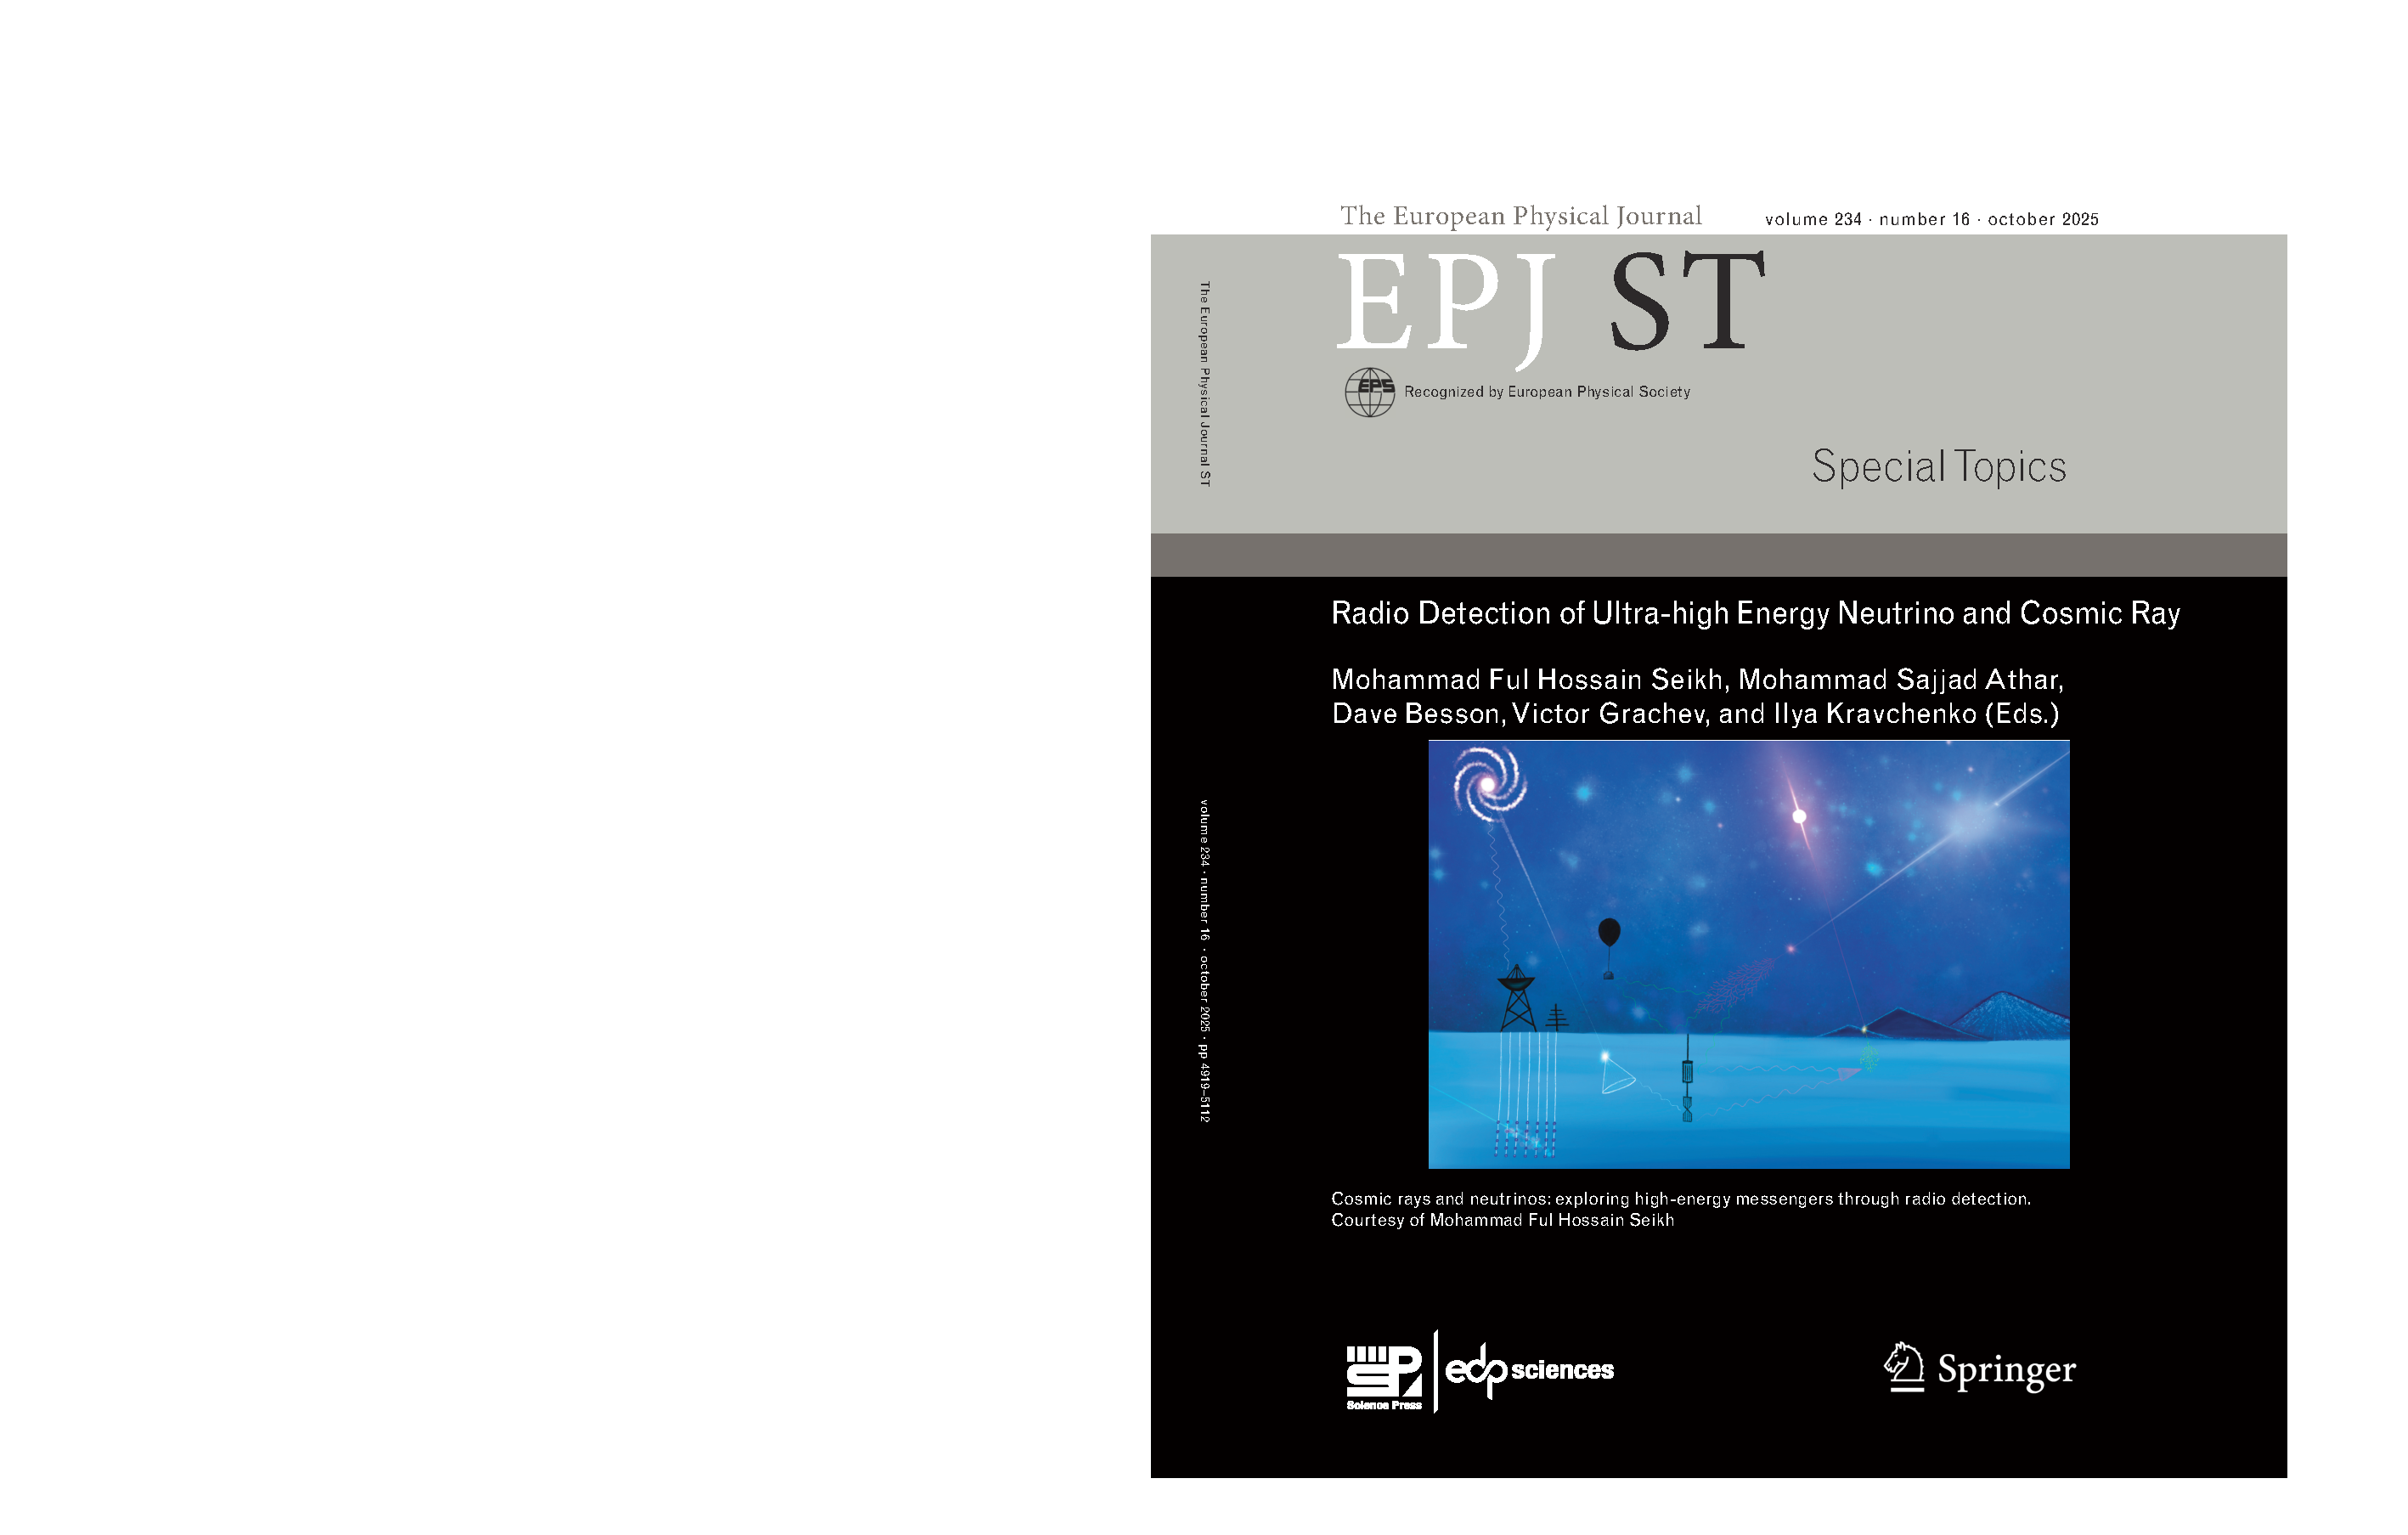
\includepdf[pages=1,pagecommand={\hypertarget{appendixpage}{}}, width=\textwidth]{Cover.pdf}

\end{document} 